\section{Approach}
\label{sec:approach}
In this section, we describe the approach to get pseudo summaries, 
%which are the ground truth of extractor's output and abstractor's input,
the ext-abs framework
with keyword-based extractor and abstractor, and RL.

\subsection{Set-level Matching Heuristics}
In order to enhance the alignment between pseudo summaries and reference summaries,
we propose a set-level method to obtain
pseudo summaries based on keywords at data preprocessing.

We use TextRank algorithm~\cite{TextRank04}
to extract keywords from reference summaries
and obtain pseudo summaries by Algorithm \ref{alg:alg}.
\begin{algorithm}[th]
\caption{Extraction of Pseudo Summaries}
\scriptsize
\label{alg:alg}
\KwIn{a source document $d$ and reference summary $s$, consisting of sentences, and keywords $k$ }
\KwOut{pseudo summary $p$ and merged reference summary $m$}
1. $len$ computes the number of sentences in a text. \\
2. $rec$ and $f1$ compute ROUGE-2 recall and F1 score between two texts. \\
3. $o$ computes the number of overlapping words two sequence. \\
%$p \leftarrow \phi$; $$
\For{$i = 0 \to len(s)$}{
     $k_i$ is the keywords of $s_i$. \\
     %Initialize $sub\_p$ by adding in $init \in D$ with highest $rec(init, s_i)$\\
     Initialize $sub\_p \leftarrow init \in d$ with highest $rec(init, s_i)$\\
     $max\_o \leftarrow o(init, s_i)$, $max\_f1 \leftarrow f1(init, s_i)$ \\
     $d' \leftarrow d-init$, $sub\_s \leftarrow s_i$ \\
     \For{$j = 0 \to len(d)$}{
	    \If{$o(d'_j,k_i) > max\_o$ \textbf{or}
		($o(d'_j,k_i) = max\_o$ \textbf{and} $f1(d'_j, s_i) > max\_f1$)}{
            $sub\_p \leftarrow sub\_p \cup \{d'_j\}$ \\
			$max\_o \leftarrow o(sub\_p, k_i)$ \\
            $max\_f1 \leftarrow f1(sub\_p, s_i)$ \\
		}
	}
    $d' \leftarrow d' - sub\_p$ \\
    \For{$j = 0 \to len(d')$}{
		\If{$f1(d'_j, s_i) > max\_f1$}{
            $sub\_p \leftarrow sub\_p \cup \{d'_j\}$ \\
            $max\_o \leftarrow o(sub\_p, k_i)$ \\
			$max\_f1 \leftarrow f1(sub\_p, s_i)$ \\
        }
    }
	Add $sub\_p$ and $sub\_s$ into $p$ and $m$ respectively. \\
    \While{\textup{the last two sub-sets in} $p$ \textup{have overlap}}
    {
        Merge last two sub-sets in $p$ and $m$ respectively.
	}
    %\If{The last set of $p$ and $sub\_p$ overlap}{
    %   $sub\_p \leftarrow sub\_p \cup$ the last set of $p$ \\
    %   $m \leftarrow m - $the last set of $m$ \\
	%}
}
\textbf{return $p$, $m$} \\
\end{algorithm}
For instance, 
we extract the sentence sets covering the most reference keywords (bold) with the highest ROUGE-2 scores
from the source document for each reference sentence. Then, if there is an overlap in the extracted sentence sets, the sets and their reference sentences will be merged.
As shown in \tabref{tab:example},
the 1st reference sentence matches source sentence $[1]$,
and the best matching for the 2nd reference sentence is the combination of source sentence $[1]$ and $[2]$. 
The pseudo summary set consisting of source sentence $[1]$ and $[2]$
is corresponding to the combination of 1st and 2nd reference sentence. 
%There is an overlap in the extracted sentence sets of first two reference, 
%the sets and these two reference sentences will be merged.
%As the matching sets of first two reference sentences have overlap,
%we merge the matching sets as well as the first two reference sentences,

%we use a greedy approach to
%add one sentence at a time to the set for a reference sentence, \textit{sub_p}, 
%such that the current set covers the most keywords.
%If there are some sentences with the same number of covered keywords,
%we select the sentence with highest ROUGE-2 recall and F1 scores.
%We stop when none of the remaining candidate
%sentences improves the keywords coverage and ROUGE scores 
%upon addition to the current summary set.
\begin{table}[th]
\begin{center}
\scriptsize
\begin{tabular}{|l|}%{|p{7cm}|rl|}
\hline \bf Set-level Pseudo Summary\\
\hline \textit{Set 1.} federal \textbf{education minister} smriti irani was visiting a \textbf{fabindia}\\
       outlet in the tourist resort state of goa on friday when she discovered a \\
	   surveillance \textbf{camera} pointed at the \textbf{changing room}. state \textbf{authorities} \\ 
	   found an overhead \textbf{camera} that the minister had spotted and determined \\
	   that it was indeed able to take \textbf{photos} \\
	   %\textit{Set 2.} four employees of the store have been \textbf{arrested}. if \textbf{convicted}, \\
	   %they could spend up to \textbf{three years} in jail. \\
\hline \bf Merged Reference Summary \\
\hline \textit{Set 1.} federal \textbf{education minister} smriti irani visited a \textbf{fabindia} store \\
       in goa , saw \textbf{cameras} . \textbf{authoroities} discovered the \textbf{cameras} could capture \\
	   \textbf{photos} rom the store 's \textbf{changing room}. \\
	   %\textit{Set 2.} the four store workers \textbf{arrested} could spend \textbf{three years} \\
	   %each in prison if \textbf{convicted} . \\
\hline
\end{tabular}
\end{center}
\caption{\label{tab:data} Set-level pseudo summary and merged reference summary of \tabref{tab:example}.}
\end{table}

\subsection{Keyword-based Extractor (KE)}

In extractive summarization,
we take the source document $D = (d_0, d_1, ..., d_n)$ as input and set-level 
pseudo summary $P = (p_0, p_1,...,p_m)$ as output.
$d$ and $p$ respectively denote the document sentence and multi-sentence set.

We propose an extractor consisting of document encoder, keywords encoder,
and a pointer network decoder.
The document encoder learns sentence representations with two options:
training from scratch with BiLSTM document encoder and fine-tuning on pretrained model named 
HIBERT.
Keywords encoder learns keywords representations
and guides the decoder to select more accurate sentences.
 %We tried two options for document encoder: BiLSTM and HIBERT
%As pretrained model can enhance the language understanding, 
%we  fine-tune our document encoder on HIBERT~\cite{HiBert19} besides BiLSTM document encoder.
The model is illustrated in \figref{fig:model}.

\begin{figure*}[th]
    \centering
    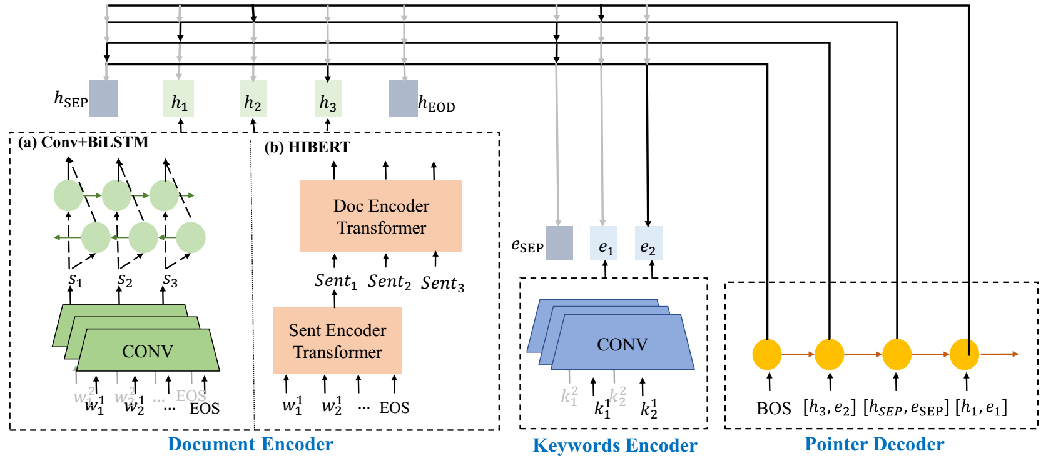
\includegraphics[width=0.8\linewidth]{model}
    \caption{The architacture of baseline model and pretrained model for key-word based extractor. }
    \label{fig:model}
\end{figure*}

%In extractive summarization,
%We take the source document $D = (d_0, d_1, ..., d_n)$ and set-level 
%pseudo summary $P = (p_0, p_1,...,p_{m})$ as output.
%$d$ denote the sentence in source document.
%Each $p$ is a set of sentences.
%Our goal is that the selected sentences 
%from source document are the same as pseudo summary at sentence-level and set-level.

\textbf{BiLSTM Document Encoder.}
The BiLSTM encoder has two sub-encoders: sentence encoder based on temporal convolutional (CNN) 
neural network and document encoder based on bidirectional LSTM network. 
The document is represented as $(h_0, h_1,...,h_n)$ where $h_i = [\overrightarrow{h_i};\overleftarrow{h_i}]$ is the representation of $i$-th sentence.
%sentence encoder and document encoder.
%We take a temporal convolutional (CNN) model as sentence encoder which 
%gets sentence vectors of $D$ by encoding the word sequences. 
%%The CNN-based sentence vectors source document become $(s_0,s_1,...,s_n)$
%Then, we take these sentence vectors as the input to 
%a bidirectional LSTM network% which is the document encoder
%learning sentence representations given their surrounding sentences as context.
%The document representation based on BiLSTM encoder is represented as
%$(h_0, h_1,...,h_n)$,
%and the representation of $i$-th sentence is $h_i = [\overrightarrow{h_i};\overleftarrow{h_i}]$ 

\textbf{HIBERT Document Encoder.}
%As the pretrained models can generate very strong sentence representations,
%we utilize the HIBERT encoder and fine-tune it on the training set 
%consisting of source documents and pseudo summaries.
%
HIBERT is a pretrained encoder~\cite{HiBert19},
which contains two Transformer-based sub-encoders.
We combine the word embeddings and their corresponding position embeddings as the input and obtain the context sensitive sentence
representations $(h'_0, h'_1,...,h'_n)$ as the output.
%to
%get the input vectors of sentence encoder.
%The sentence encoder transforms the inputs
%into a list of hidden representations $(x_0, x_1,...,x_{|d_i|})$. 
%We take the $t_i = x_{|d_i|}$
%as the representation of sentence $d_i$.
%The document encoder is a 
%Transformer applied on the sentence level.
%We obtain the context sensitive sentence representations $(h_0, h_1,...,h_n)$
%by running the Transformer on sentence representations 
%$(t_0, t_1,..., t_n)$, 

\textbf{Keywords Encoder.} 
We use TextRank algorithm to 
receive a sequential list of keywords from source document, 
arranged based on their locations in source. 
We take CNN model to embed extracted keywords as $(e_0, e_1, ..., e_k)$.
The combination of keywords representation and sentence representation
emphasizes the keywords regarded as salient information
and makes model consider them during sentence selection.
%of source document.

\textbf{Pointer Decoder.} 
%Based on the document representations and keywords representation from encoders,
We use Pointer Network~\cite{PointNet15} as the decoder.
%to extract sentence from source document.
Our pseudo summaries are supervised signal of the decoder, which is a sequence of multi-sentence sets.
We extract a set of keywords for each multi-sentence set in pseudo summaries and arrange them
based on their location in the text.
%The pseudo keywords also consists of 
%multi-keywords sets.
To distinguish the sentences and keywords in different sets, 
we set the representations for the
placeholder $<$SEP$>$ in pseudo summaries and pseudo keywords.% during decoding.
The ground truth sentence selection labels of a pseudo summary is
$\textbf{Y} = (Y_0,Y_1,...,SEP,...,Yn)$.
The pseudo keywords of a summary becomes $\textbf{K} = (K_0,K_1,...,SEP,...,K_m)$.
We randomly initialize the representation of $h_{SEP}$ and $e_{SEP}$. 

At each time step $t$, we take the output of decoder attending to the encoder sentence representations as predicted vector $c^h_t$, which is calculated by:
%\begin{small}
\begin{equation}
\small
\begin{aligned}
\small
c^h_t &= \sum_{i}^{n} {\alpha_{it}^h W^{a1} h_i} \\
\alpha_t^h &= softmax(v^h \tanh(W^{r1} r_t + W^{h1} h_i)) \\ 
\end{aligned}
\end{equation}
%\end{small}
where $r_t$ is the decoder hidden state at step $t$.
$h_i$ is the sentence representation of $i$-th sentence
based on document encoder (BiLSTM or HIBERT).
$a_t^h$ is the attention weights based on sentences.
$W$ and $v$ in different labels are trainable parameters.
Similarly, the keywords vector $c_t^e$ can be computed.
% as follows:
%\begin{equation}
%\small
%c_t^e = \sum_{j}^{m} {\alpha_{jt}^e W^{a2} e_j} \\
%\end{equation}
%\begin{equation}
%\small
%\alpha = softmax(a_t^e)
%\end{equation}
%\begin{equation}
%\small
%a_{jt}^e = v^h \tanh(W^{r2} r_t + W^{e1} e_j) \\
%\end{equation}
%where $h_i$ is the document representation of $i$-th sentence.
%Both $h_{SEP}$ and $e_{SEP}$ participate the calculation.
We compute the current extraction probabilities
using predicted sentence vector and keywords vector:
%\begin{small}
\begin{equation}
\small
\begin{aligned}
p(y_t|y_1,..,y_{t-1}) = softmax(v \tanh(W^{r} r_{t}  +& W^{h} c_t^h  \\
                                                     +& W^{e} c_t^e))
\end{aligned}
\end{equation}
%\end{small}
%where $y_t$ is the lable of sentence with the highest probability.
where $y_t$ is the sentence with the highest probability at current step.

\textbf{Combinational Loss.} 
We propose a combinational loss to train extractor, including
cross-entropy loss, keywords loss and set loss.
The {\em cross-entropy loss} reflects the accuracy of one-to-one alignment between
extracted sentences and pseudo summaries (ground truth).
which is computed as:
\begin{equation}
\small
L_{ce} = - \sum_{(Y,D) \in T}{\log(p(Y|D))}
\end{equation}
%where $Y$ is the ground truth and $D$ is source document.
where $T$ is training set with $N$ samples.
We use {\em keywords loss} to emphasize the importance of the related salient information.
%can deal with the incorrect selection causing by
%the generated sentence representation which are similar to the 
%ground truth but without salience information based on keywords.
The probability of keywords extraction is computed as: 
%\begin{small}
\begin{equation}
\small
p(k_t|k_1,...,k_{t-1}) = softmax(v \tanh(W^{'r} r_{t} + W^{'e} c_t^e)) 
\end{equation}
%\end{small}
where $k_t$ is the predicted keyword at $t$ step.
We compute the keywords loss based on the keywords ground truth $K$ 
and source document $D$ as:
%\begin{small}
\begin{equation}
\small
L_{key} = - \sum_{(K,D) \in T}{\log(p(K|D))}
\end{equation}
%\end{small}
In order to abstract the extractor output consisting of multi-sentence sets
to generate a final summary,
we need correctly predict $<$SEP$>$ at the proper positions
and sentences in each set.
Thus, we define the {\em set loss} function as
\begin{equation}
\small
l_{set} = -  \sum_{(Y,D) \in T}{\log(p(Y'|D))}
\end{equation}
where $Y'$ is the predicted results of $Y$.
We align the $<$SEP$>$ of $Y$ and $Y'$
in the same position by padding or truncation 
the sequence of sentence labels in the set of $Y$.
For example, given ground truth $Y = (y_0,y_1,SEP,y_2)$ 
and predicted labels $Y' = (y'_0,SEP,y'_1,y'_2)$, we get
$Y' = (y_0,SEP,y_1,PAD)$, 

We use the combinational loss as follow:
\begin{equation}
\label{func:loss}
\small
L_{ext} = - \frac{1}{N} (\lambda_{c}L_{ce} + \lambda_{k}L_{key} + \lambda_{s}L_{set})
\end{equation}



\subsection{Abstractor}
The abstractor can paraphrase the inputs.
We take set-level pseudo summaries and their reference summaries 
as the input and output of abstractor at training.
%which is the pseudo summaries at training and the output of extractor at testing.
The abstractor is an independent neural network without parameter sharing with extractor.

In this paper, we take two representative Enc-Dec model options as our abstractor,
Base-Abs and Pre-Abs. \textbf{Base-Abs} is the standard Enc-Dec model with attention mechanism~\cite{luong15}
and copy mechanism~\cite{SeeLM17}.
%The copying mechanism help decoder
%replace the predicted word of out-of-vocabulary by
%the word with highest attention score in encoder.
%The embedding matrix
%as well as output projection matrix 
%words in the input document, follow by Paulus~\shortcite{PaulusXS17}. 
\textbf{Pre-Abs} is obtained by fine-tuning the pretrained model BART~\cite{BART19} 
on our pseudo summaries and reference summaries.
%consists of bidirectional transformer encoder and auto-Regressive transtormer decoder,
%it can be directly fine-tuned for abstractive summarization tasks and outperforms
%previous models. 

\subsection{Reinforcement Learning (RL)}
We apply RL to make ext-abs framework be an end-to-end trainable model.
%We pretrain the extractor and abstractor separately on (source document, pseudo summaries) pairs
%and (pseudo summaries, reference summaries) pairs.
%Then we fine-tune them on source documents and reference summaries through RL,
%which avoid abstractor training with irrelevant selected sentences
%and extractor with noisy reward.
We use policy gradient techniques
to optimize our model.
We take extractor as RL agent without altering the language model of abstractor~\cite{FastAbs18}.

At each training step $t$, 
we first use extractor to obtain an extracted summary, which divided into several 
sentence sets by $<$SEP$>$.
Then, the abstractor respectively
paraphrases these sets, which are connected with $<$SEP$>$ to generate a summary.
%The ROUGE scores between $<$SEP$>$ and other sentences are $0$.
%The extracted summary are divided into sentence sets by $<$SEP$>$,
%which .
%If the sentence is $<$SEP$>$, we set it as an empty sequence and take it as the end of the set. 
%\footnote{Given two sequence, if one of them is empty, the ROUGE score is $0$.
%If both are empty, the ROUGE score is $1$.}
The extracted summary $Q = (q_0^0,q_1^0,...,q_t^l,...,q_{y}^{M})$ and its pseudo summary $P = (p_0^0,p_1^0,...,p_t^l,...,p_x^m)$ 
consists of sentences.
$A = (a_0,a_1,..,a_{M})$ and $B = (b_0,b_1,..,b_m)$ denote
the generated summary of abstractor and reference summary consisting of multi-sentence sets.
$q_t^l$ means that the $t$-th sentence in summary belongs to the $z$-th sets.
$m$ denotes the number of set in pseudo summary and reference summary.
We define a {\em sentence-level} rewards as:
\begin{equation}
\small
R_{sent}(t) = ROUGE-L_{F1}(q_t,p_t)
\end{equation}
The sentence-level reward directly measure the accuracy of extracted sentence.
To align generated summary and reference summary, we propose a {\em set-level reward}.
The pseudo summary should be padded (truncated) as mentioned in {\em set loss},
$\hat{P} = (\hat{p}_0^0,\hat{p}_1^0,...,\hat{p}_{y}^M)$
We set ROUGE-2 as $R$-$2$. 
The set-level reward is computed as:

\begin{equation}
\small
R_{set}(t) = 
	\begin{cases}
		   \mbox{$R$-$2_{recall}(a_l,b_l)$}, \quad \mbox{if $t=min(|p^l|,|\hat{p}^l|)$}\\
           \mbox{$R$-}2_{recall}(seq(q_0^l...q_t^l),b_l), \quad    \mbox{$others$}\\
   \end{cases}
\end{equation}
where $seq$ connect all the inputs together.
We use R-2 recall to judge the match between extracted sentence and reference summary.
Considering the quality of an overall generated summary,
we compute {\em summary-level reward} as:

\begin{equation}
\small
R_{summ}(t) = 
	\begin{cases}
		   \mbox{$R$-$2_{F1}(a_l,B_l)$}, \quad \mbox{if $t=min(|p^l|,|\hat{p}^l|)$}&\\
           \mbox{$R$-}2_{F1}(seq(q_0^0...q_t^l),B), \quad \mbox{$others$}&\\
   \end{cases}
\end{equation}

The total reward is the combination of above:

\begin{equation}
\label{func:reward}
\small
R_{overall} = \gamma_{1}R_{sent} + \gamma_{2}R_{set} + \gamma_{3}R_{summ}
\end{equation}



